\documentclass{article}
\usepackage[utf8]{inputenc}
\usepackage[italian]{babel}
\usepackage{amsmath}
\usepackage{amssymb}
\usepackage{siunitx}
\usepackage{tabularray}
\usepackage{graphicx}
\usepackage{float}
\usepackage{xfrac}
\newcommand*{\diam}{\varnothing}
\newcommand*{\best}[1]{{#1}_\text{best}}
\newcommand*{\bestp}[1]{{\left(#1\right)}_\text{best}}
\newcommand*{\pbest}[1]{\left({#1}_\text{best}\right)}
\newcommand*{\pbestp}[1]{\left({\left(#1\right)}_\text{best}\right)}
\newcommand*{\errrel}[1]{\frac{\delta #1}{{#1}_\text{best}}}
%% <custom footnotes/>
%\newcounter{savefootnote}
%\newcounter{symfootnote}
%\newcommand{\symfootnote}[1]{%
%   \setcounter{savefootnote}{\value{footnote}}%
%   \setcounter{footnote}{\value{symfootnote}}%
%   \ifnum\value{footnote}>8\setcounter{footnote}{0}\fi%
%   \let\oldthefootnote=\thefootnote%
%   \renewcommand{\thefootnote}{\fnsymbol{footnote}}%
%   \footnote{#1}%
%   \let\thefootnote=\oldthefootnote%
%   \setcounter{symfootnote}{\value{footnote}}%
%   \setcounter{footnote}{\value{savefootnote}}%
%}
%% </custom footnotes>
\title{
    Laboratorio di Fisica 1\\
    R3: Misura del modulo del campo gravitazionale locale
}
\author{Gruppo 17: Bergamaschi Riccardo, Graiani Elia, Moglia Simone}
\date{18/10/2023 – 25/10/2023}
\makeindex
\begin{document}

\maketitle

\begin{abstract}
    Il gruppo di lavoro ha misurato indirettamente il modulo del campo gravitazionale locale ($\vec{g}$) con due metodi distinti:
    dapprima facendo cadere due palline da ferme, successivamente tenendo conto di distanze diverse e velocità iniziali diverse.
\end{abstract}

\setcounter{section}{-1}  % Count sections starting from 0
\section{Materiali e strumenti di misura utilizzati}
\begin{center}
    \begin{tblr}{ |Q[l,m]|Q[c,m]|Q[c,m]|Q[c,m]| }
        \hline
        \textbf{Strumento di misura} & \textbf{\:\:\:\:\:Soglia\:\:\:\:\:} & \textbf{Portata} & \textbf{Sensibilità} \\
        \hline
        {Due fototraguardi con \\ contatore di impulsi} & \qty{1}{\micro s} & \qty{99999999}{\micro s} & \qty{1}{\micro s} \\
        \hline[dashed]
        Metro a nastro & \qty{0.1}{cm} & \qty{300.0}{cm} & \qty{0.1}{cm} \\
        \hline[dashed]
        Micrometro ad asta filettata & \qty{0.01}{mm} & \qty{25.00}{mm} & \qty{0.01}{mm} \\
        \hline
        \hline
        \textbf{Altro} & \SetCell[c=3]{l} \textbf{Descrizione/Note} \\
        \hline
        {Sistema di sgancio \\ elettropneumatico} & \SetCell[c=3]{l} {
            Usato, tramite comando manuale, per \\
            rilasciare le sferette in modo riproducibile.
        } \\
        \hline[dashed]
        Livella & \SetCell[c=3]{l} {
            Utile per assicurarsi che i fototraguardi \\
            siano orizzontali.
        } \\
        \hline[dashed]
        Due sferette & \SetCell[c=3]{l} {Le chiameremo $A$ e $B$.} \\
        \hline
    \end{tblr}
\end{center}

\section{Caduta libera dallo stato di quiete}
\subsection{Esperienza e procedimento di misura}
\begin{enumerate}
    \item
        Misuriamo con il metro a nastro la distanza $d_0$ tra il centro
        del pistone del sistema di sgancio e un fototraguardo e con il
        micrometro ad asta filettata i diametri $\diam_A,\diam_B$ delle
        due sferette.\\
        Nel nostro caso, $d_0 = \left(125.8\pm 0.3\right)\unit{cm}$.\\
        \emph{
            \textbf{Nota.} Il gruppo di lavoro ha stimato
            $\delta d_0 = \qty{0.3}{cm}$ nonostante la sensibilità
            del metro sia notevolmente inferiore, a causa della difficoltà
            nel determinare il centro del pistone e la posizione precisa del
            fascio a infrarossi del fototraguardo.
        }
    \item
        Acceso e impostato adeguatamente il contatore di impulsi,
        misuriamo 100 volte il tempo di caduta di ogni sferetta
        $s\in\left\{A;B\right\}$
        fra il sistema di sgancio e il fototraguardo.
\end{enumerate}

\emph{
    \textbf{Notazione.} Indicheremo con $\left(t_s\right)_i$
    ogni $i$-esima misura del tempo di caduta
    $\left(i\in\left[0;100\right)\cap\mathbb{N}\right)$,
    mentre con $\overline{t_s}$ il tempo di caduta medio.
    In particolare:\[
        \delta\!\left(\overline{t_s}\right) = \sigma_{\overline{t_s}} =
        \frac{\sigma_{t_s}}{\sqrt{100}}   = \frac{\sigma_{t_s}}{10}.
    \]
}


\emph{
    \textbf{Osservazione.} Poiché il pistone tiene ferma la sferetta
    per la parte centrale, mentre il fototraguardo rileva il passaggio
    della pallina nel momento in cui il suo punto più basso interrompe il
    fascio di luce (infrarossa), la distanza percorsa dalla sferetta $s$
    nel tempo misurato non sarà semplicemente $d_0$, bensì
    $d_0 - \frac{1}{2}\diam_s$.
}

\subsection{Analisi dei dati raccolti e conclusioni}
Fissato un sistema di riferimento solidale all'apparato di misura, con origine
nella posizione di partenza delle sferette e $\hat{x} = \hat{g}$, possiamo
scrivere la seguente legge del moto:
\[x(t) = \frac{1}{2}g t^2\]
La norma di $\vec{g}$ misurata indirettamente è allora ricavabile da:
\begin{equation}\label{eq:1}
    g_s = \frac{2d_0 - \diam_i}{\left(\overline{t_s}\right)^2}
    % \best{g} = \frac{2\best{\left(d_0\right)} - \bestp{\diam_i}}
    %                 {\bestp{\overline{t_i}}^2}
    % \qquad\wedge\qquad
    % \errrel{g} = \frac{2\left(\delta d_0\right) - \delta \diam_i}
    %                   {2\best{\left(d_0\right)} - \bestp{\diam_i}}
    %            + 2\frac{\sigma_{\overline{t_i}}}{\overline{t_i}}
\end{equation}
dove l'errore su $g_s$ segue dalla propagazione degli errori su $d_0,\diam_s$ e
$\overline{t_s}$.

Di seguito riportiamo gli istogrammi dei tempi e i valori di $g$ così ottenuti.
Per confrontare queste misure indirette ($g_A$ e $g_B$) con il valore atteso, ovvero
$g=\qty{9.806}{m\per s^2}$, valutiamo, per ogni sferetta $s$, la seguente quantità:\[
\varepsilon_s = \frac{\bestp{g_s} - g}{\delta g_s}
\] Allora la misura $g_s$ da noi ottenuta è compatibile con $g$ se e solo se
$\left|\varepsilon_s\right|\le1$; inoltre, dal segno di $\varepsilon_s$ è possibile
sapere se $g_s$ misurata è una sovrastima ($\varepsilon_s>0$) o una sottostima
($\varepsilon_s<0$).

\begin{figure}[H]
    % trim={< v > ^}
    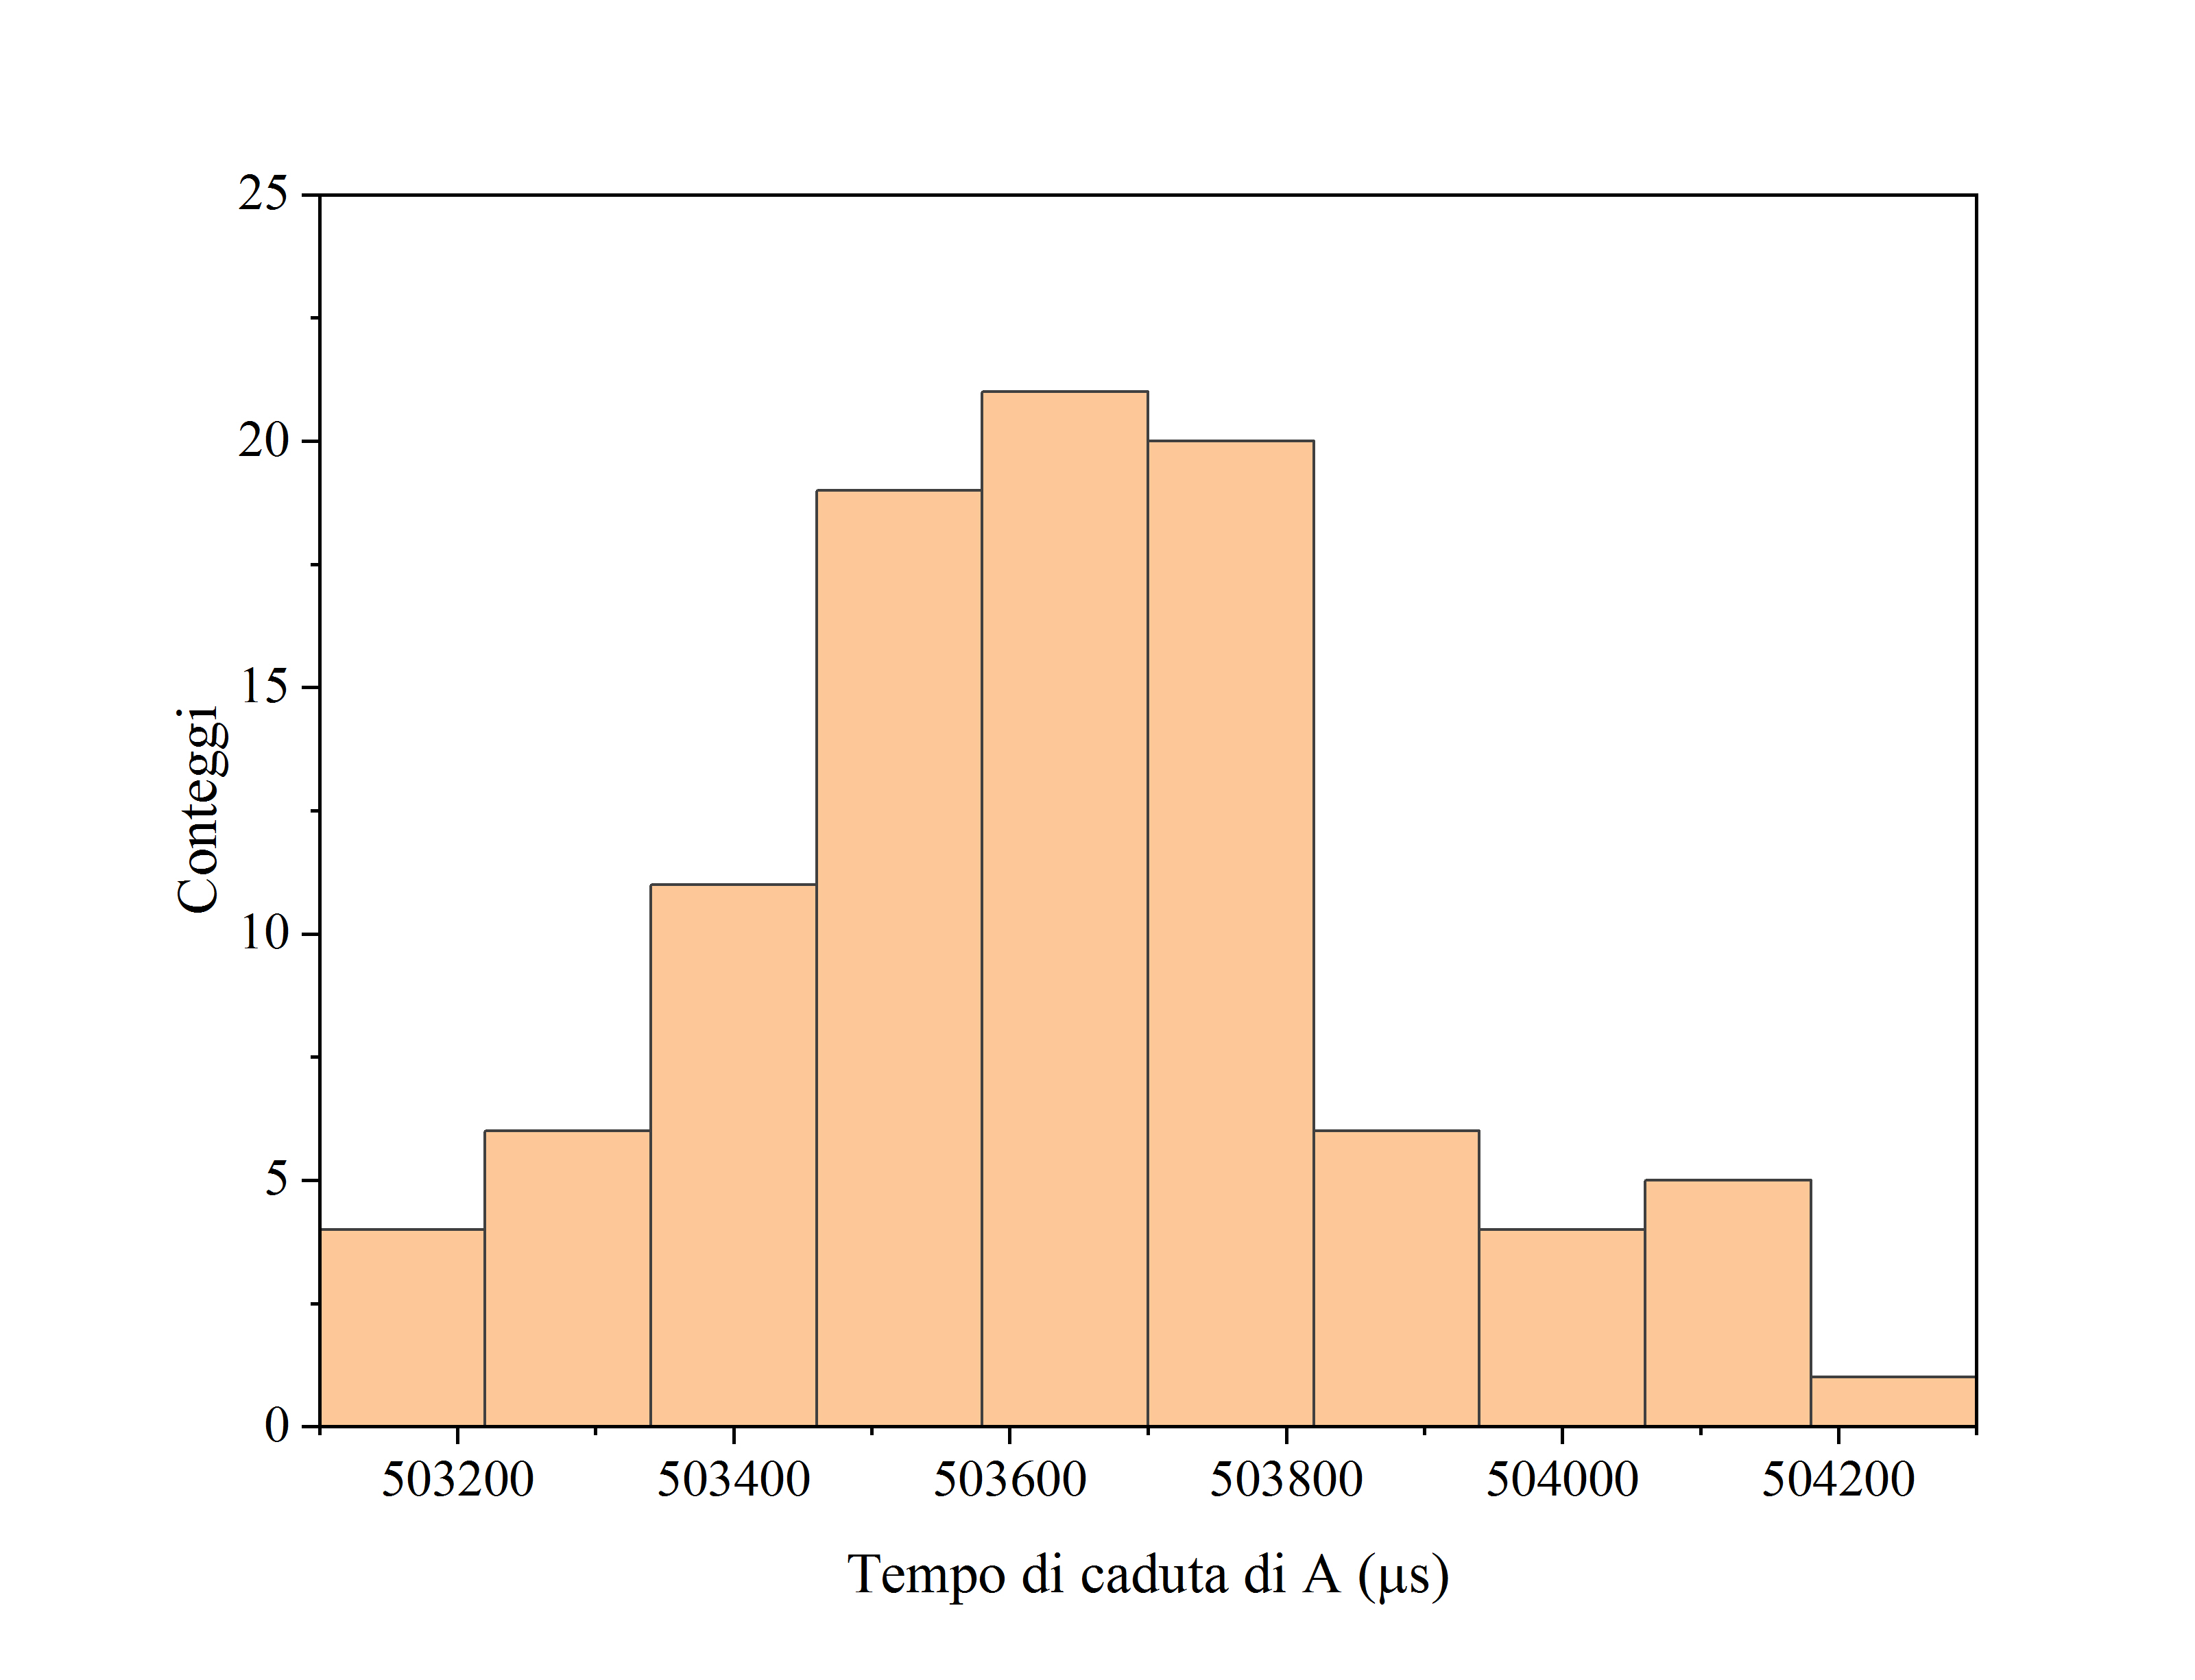
\includegraphics[trim={2cm .5cm 2.4cm 2.1cm},clip,width=.5\textwidth]{TempiA.jpg}
    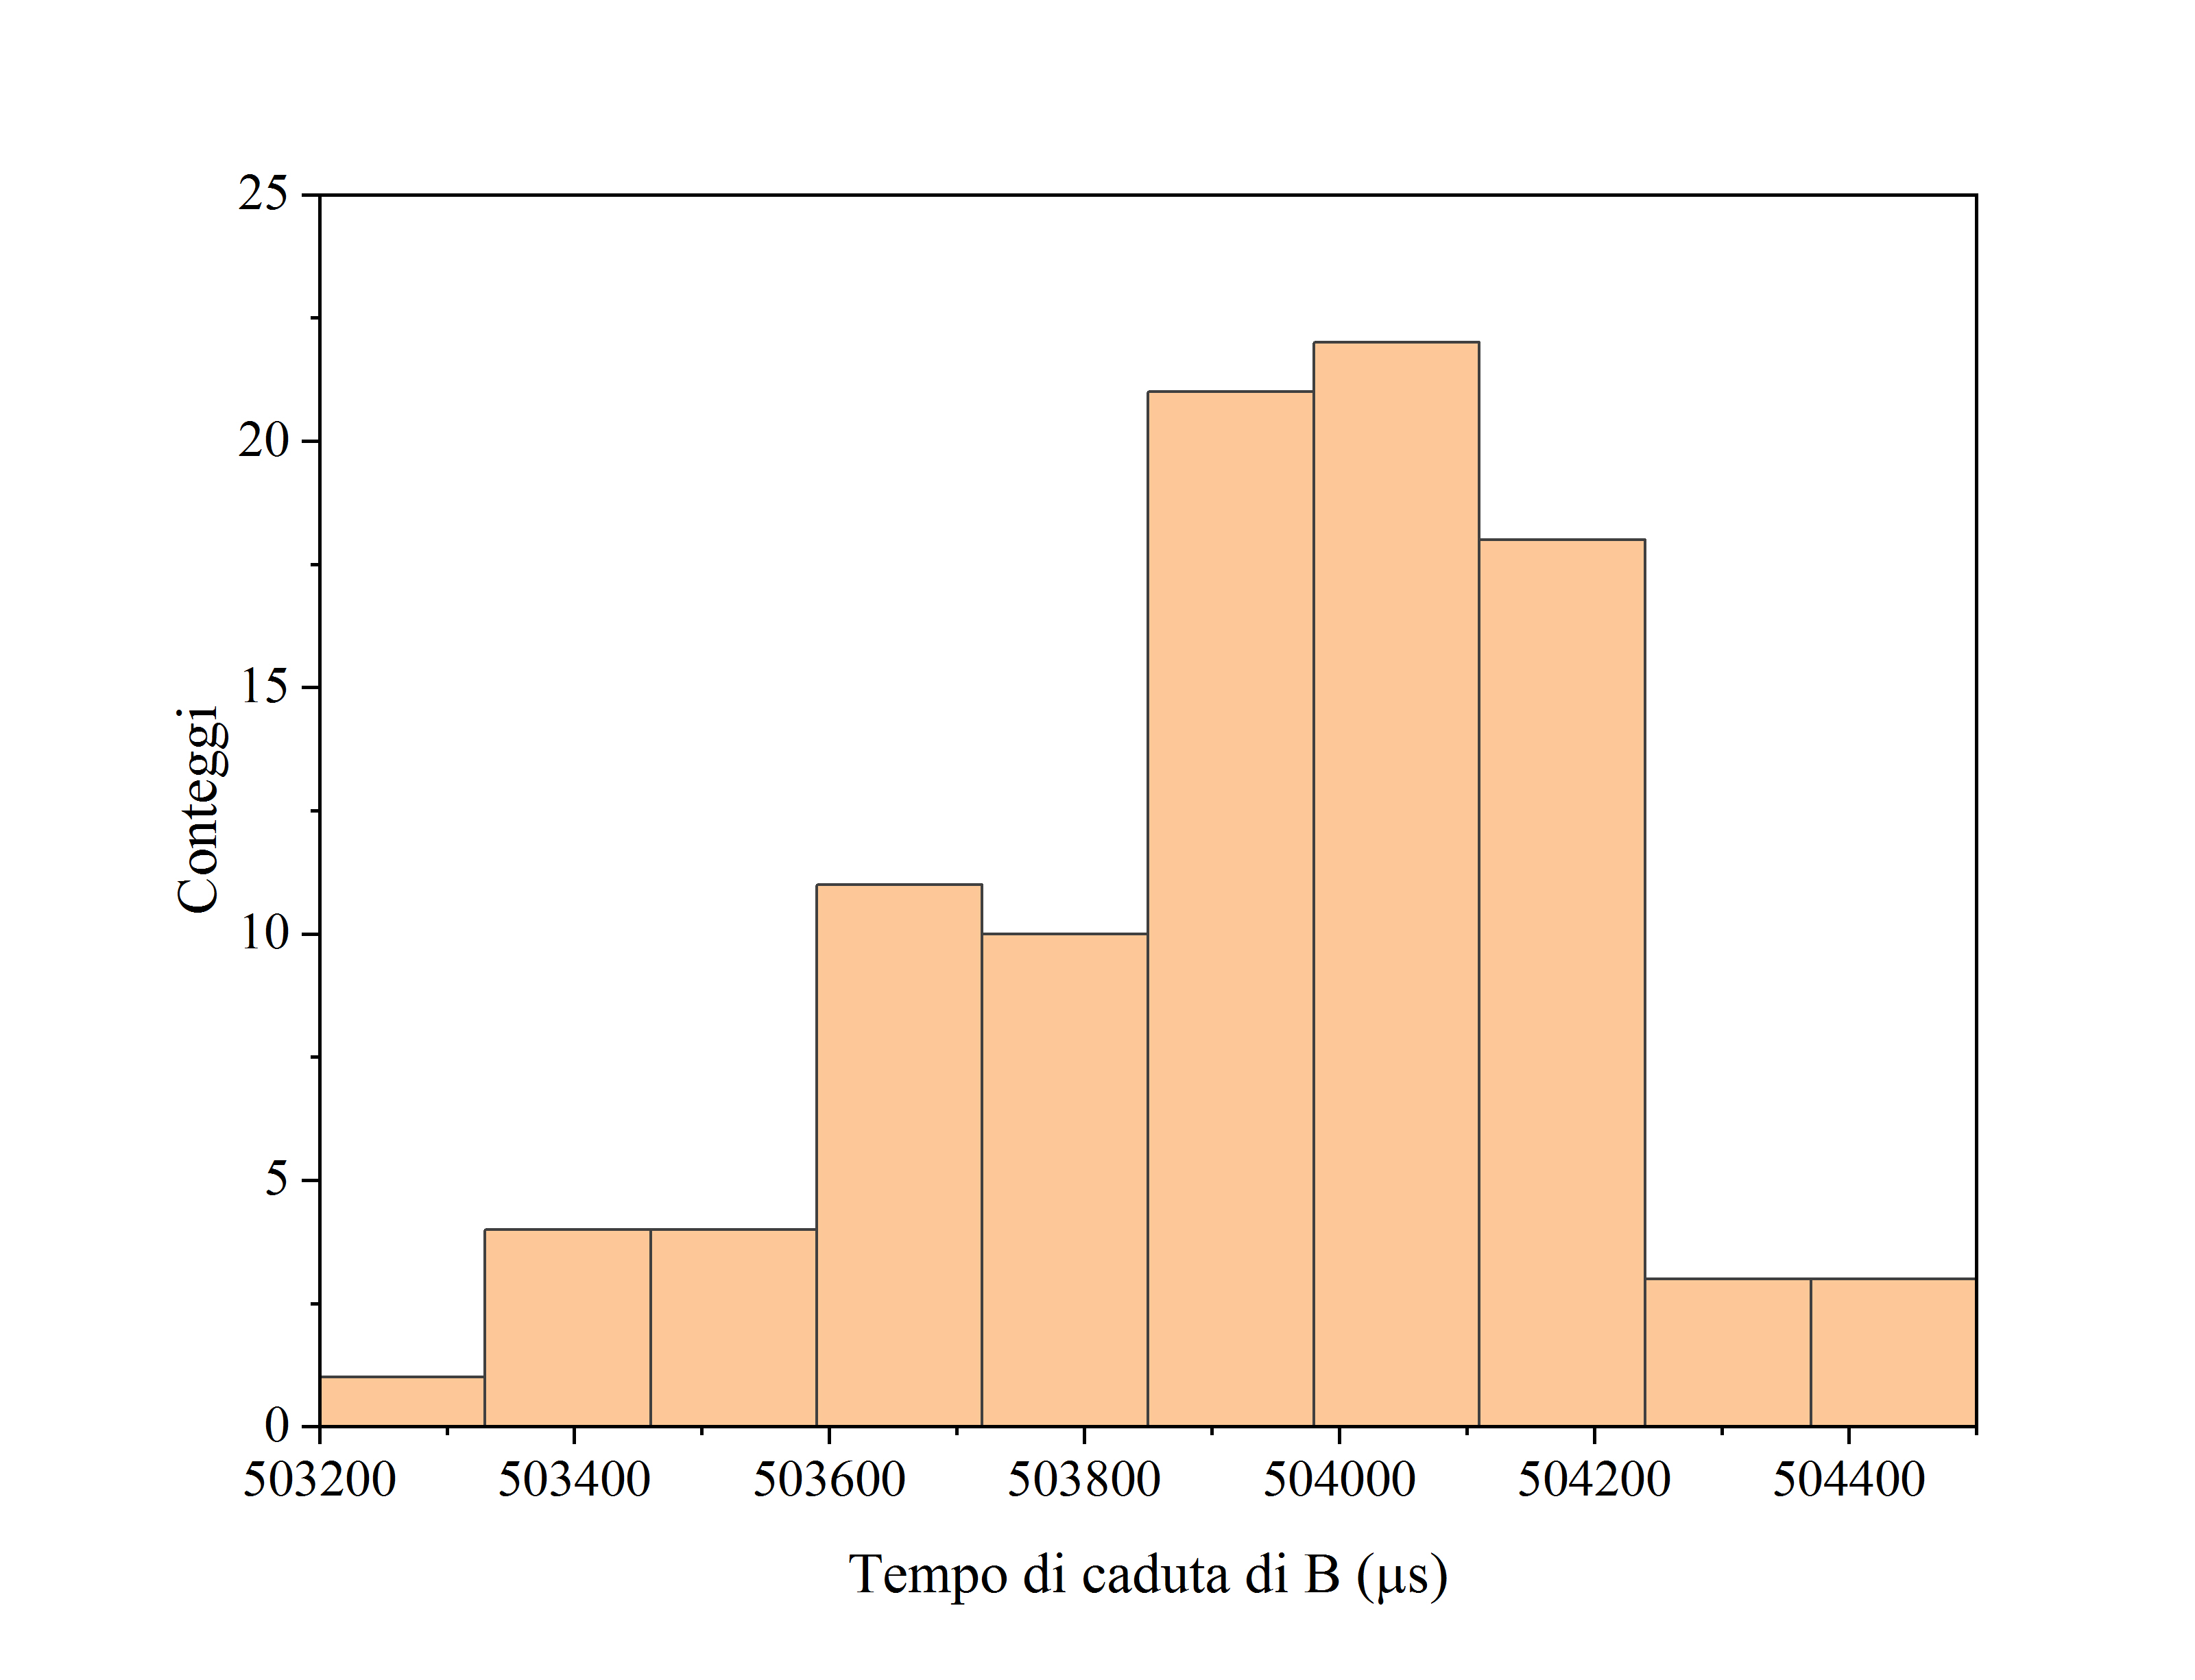
\includegraphics[trim={2cm .5cm 2.4cm 2.1cm},clip,width=.5\textwidth]{TempiB.jpg}
    \caption{Istogrammi dei dati raccolti ($t_A$ e $t_B$)}
\end{figure}
\vspace{.5cm}
\begin{center}
    \begin{tblr}{ |Q[c,m]|Q[c,m]|Q[c,m]|Q[c,m]|Q[c,m]| }
        \hline
            $s$ &
            $\diam_s\:(\unit{mm})$ &
            $\overline{t_s}\:(\unit{ms})$ &
            $g_s\:(\unit{m\per s^2})$ &
            $\varepsilon_s$ \\
        \hline
        A & $24.62\pm0.01$ & $503.63\pm0.02$ & $9.82\pm0.02$ & $+0.67$ \\
        \hline[dashed]
        B & $22.23\pm0.01$ & $503.93\pm0.02$ & $9.82\pm0.02$ & $+0.57$ \\
        \hline
    \end{tblr}
\end{center}

Le misure di $g$ ottenute sono pertanto ampiamente consistenti con il valore atteso.

\emph{
    \textbf{Osservazione.} Dai valori di $\varepsilon$ non emerge una differenza
    significativa fra le due sferette. In particolare, sembra che l'attrito viscoso
    dell'aria abbia agito in maniera trascurabile (come ci aspettavamo).\\
    Tuttavia, dopo una più attenta analisi, è comunque possibile notare una tendenza:
    in media, la sferetta con raggio maggiore ha percorso la stessa distanza in un
    tempo leggermente minore.
    Pertanto, ciò potrebbe suggerire un effetto molto ridotto dell'attrito dell'aria;
    questa tendenza però non è rispecchiata dai valore di $\varepsilon$,
    probabilmente a causa di una sovrastima della distanza $d_0$. Si noti infatti che
    dal segno degli $\varepsilon$, entrambe le misure di $g$ sono risultate sovrastime,
    mentre, nell'equazione (\ref{eq:1}), $d_0$ è al numeratore.
}

\section{Caduta libera con velocità iniziale}
\subsection{Esperienza e procedimento di misura}
Ripetiamo 5 volte i seguenti passaggi (con $i\in\left[1;5\right]\cap\mathbb{N}$):
\begin{enumerate}
    \item
        Spostiamo il secondo fototraguardo ad una distanza dal primo a piacere;
        misuriamo poi con il metro a nastro tale distanza $d_i$.\\
        \emph{
            \textbf{Nota.} A differenza di prima, stavolta non ci sono state
            particolari difficoltà relativi alla misura di $d_i$; di conseguenza,
            il gruppo di lavoro ha utilizzato $\delta d_i = \qty{1}{mm}$, ovvero
            la sensibilità dello strumento.
        }
    \item
        Acceso e impostato adeguatamente il contatore di impulsi, sganciamo la
        sferetta $A$ e ne misuriamo 50 volte il tempo di caduta fra i due
        fototraguardi.
\end{enumerate}

\emph{
    \textbf{Notazione.} Indicheremo con $\left(t_i\right)_j$
    ogni $j$-esima misura del tempo di caduta lungo l'$i$-esima distanza
    $\left(j\in\left[0;50\right)\cap\mathbb{N}\right)$,
    mentre con $\overline{t_i}$ il tempo di caduta medio.
    In particolare:\[
        \delta\!\left(\overline{t_i}\right) = \sigma_{\overline{t_i}} =
        \frac{\sigma_{t_i}}{\sqrt{50}} = \frac{\sigma_{t_i}}{5\sqrt{2}}.
    \]
}


\emph{
    \textbf{Osservazione.} Poiché i due fototraguardi registrano l'evento
    del passaggio della pallina allo stesso modo, la distanza percorsa dalla
    pallina nel tempo $\overline{t_i}$ è semplicemente $d_i$.\\
    Inoltre, poiché il primo fototraguardo rimane fisso, la velocità iniziale
    $v_0$ della pallina resta costante durante tutto l'esperimento.
}

\subsection{Analisi dei dati raccolti e conclusioni}
Fissato un sistema di riferimento solidale all'apparato di misura, con origine
nella posizione del primo fototraguardo e $\hat{x}=\hat{g}$, possiamo scrivere
la seguente legge del moto:
\[x(t) = \frac{1}{2} g t^2 + v_0 t\]
Possiamo linearizzare questa equazione dividendo ambo i membri per $t$:
\[\frac{x(t)}{t} = \frac{1}{2} g t + v_0\]
Nei termini delle nostre misure:
\begin{equation}\label{eq:2}
    \frac{d_i}{t_i} = \frac{1}{2} g t_i + v_0
\end{equation}

\emph{
    \textbf{Osservazione.} $d_i/t_i$ è, per definizione, la velocità
    media $\left(v_m\right)_i$ della sferetta nell'intervallo di tempo $t_i$.
}

Per determinare $g$ e $v_0$, possiamo semplicemente effettuare una regressione
lineare (pesata\footnote{
    L'utilizzo del metodo pesato è giustificato dal fatto che l'errore
    sull'ordinata non è costante, come si può osservare chiaramente sia
    dalla tabella che dal grafico della regressione lineare stessa.
}) con equazione (\ref{eq:2}). In particolare, il coefficiente angolare della
retta di regressione sarà $\frac{1}{2} g$ e l'intercetta sarà $v_0$.

Qui riportiamo gli istogrammi dei tempi misurati, seguiti da una tabella
riassuntiva e dal grafico della regressione lineare:

\begin{figure}[H]
    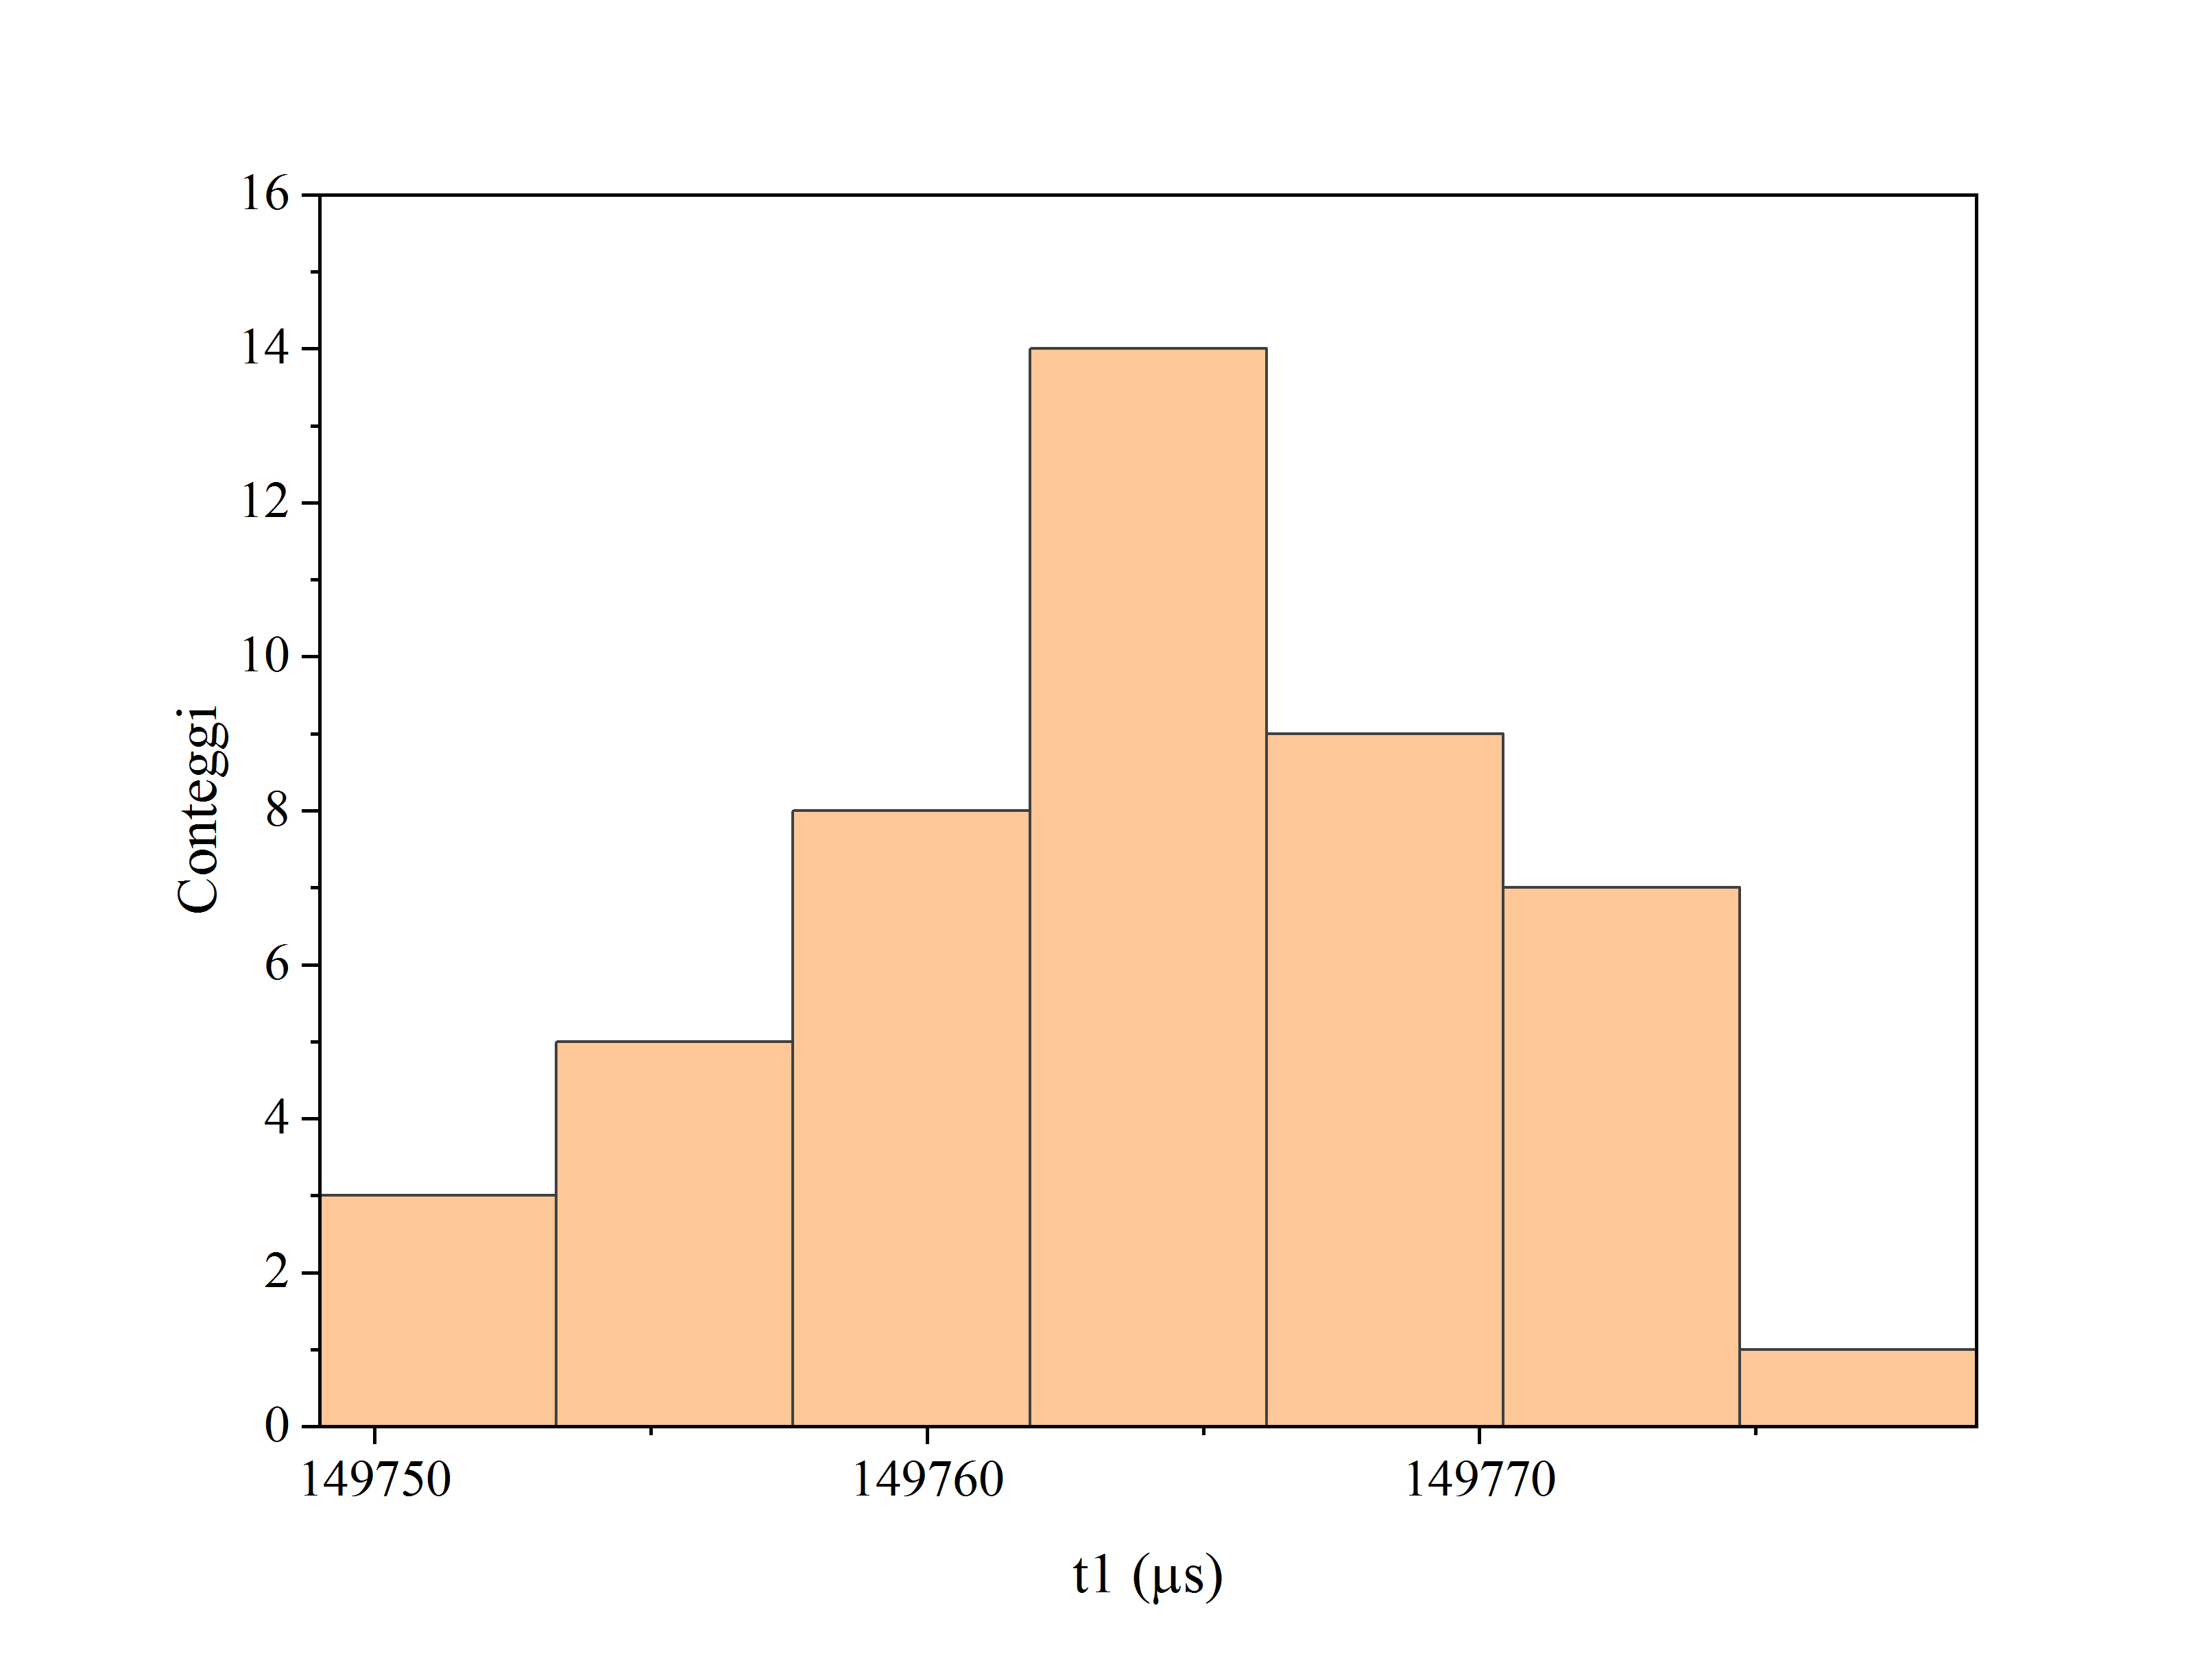
\includegraphics[trim={2cm .5cm 2.4cm 2.1cm},clip,width=.5\textwidth]{t1.jpg}
    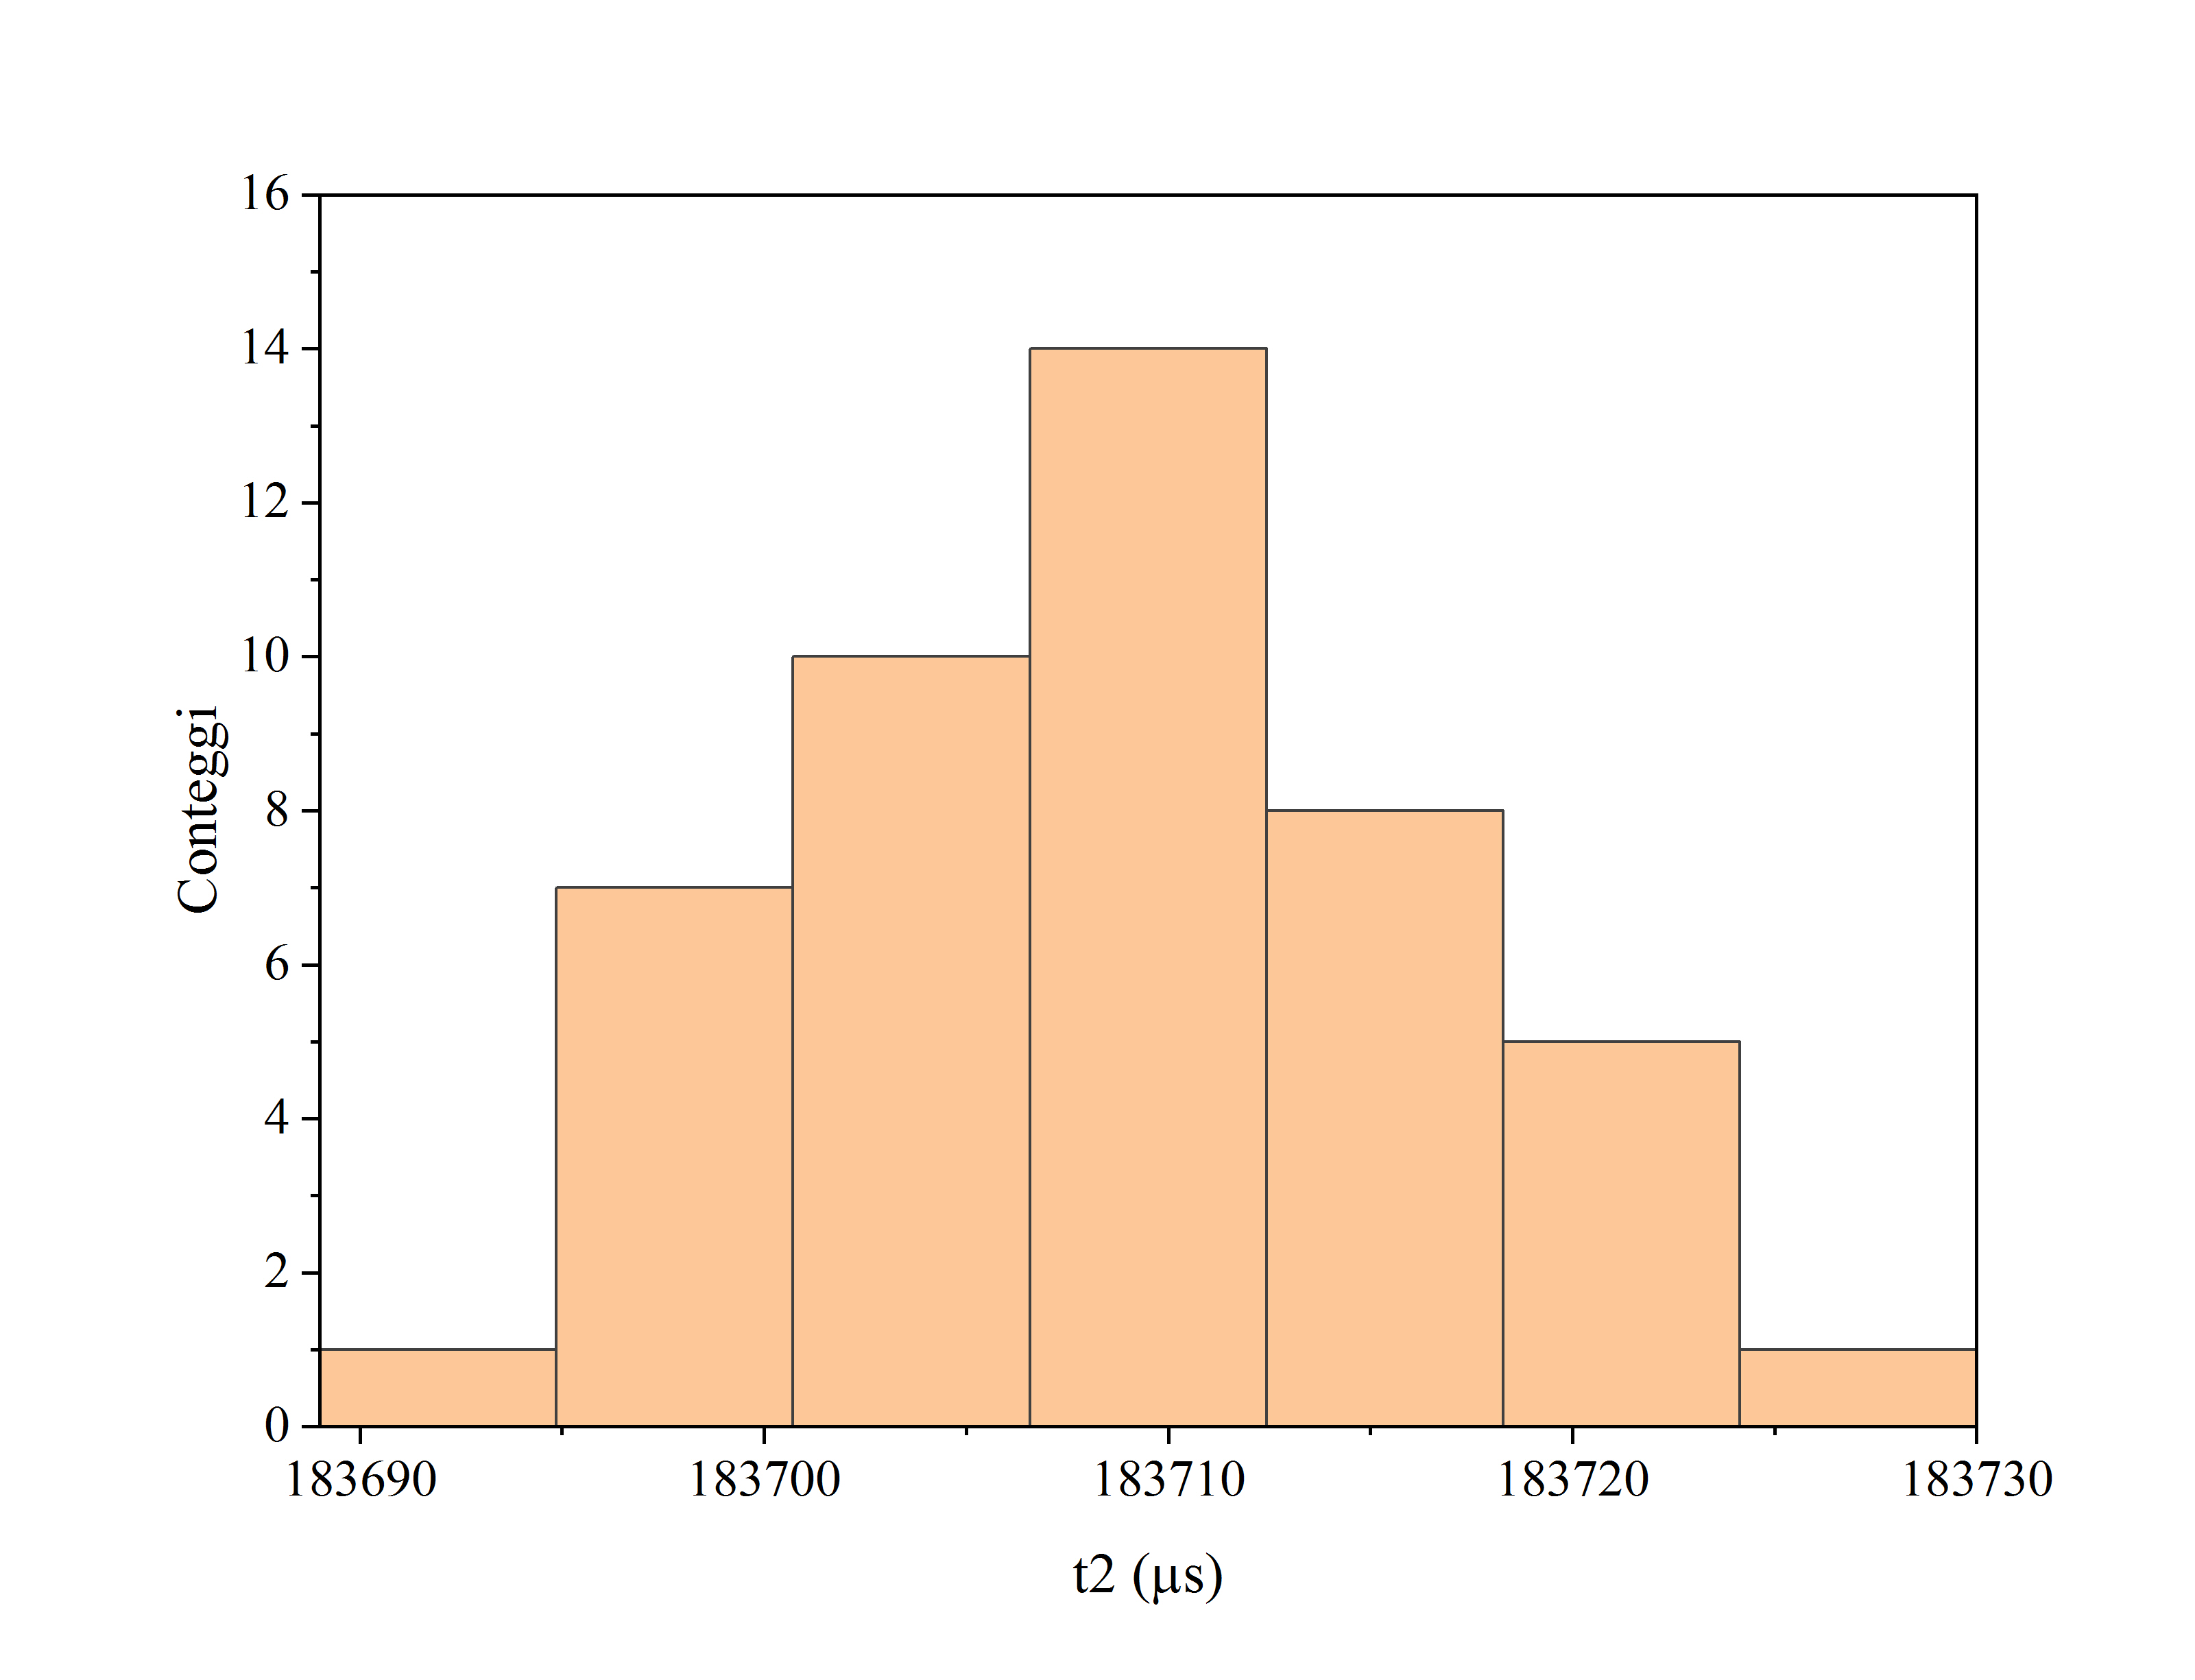
\includegraphics[trim={2cm .5cm 2.4cm 2.1cm},clip,width=.5\textwidth]{t2.jpg}
    \\
    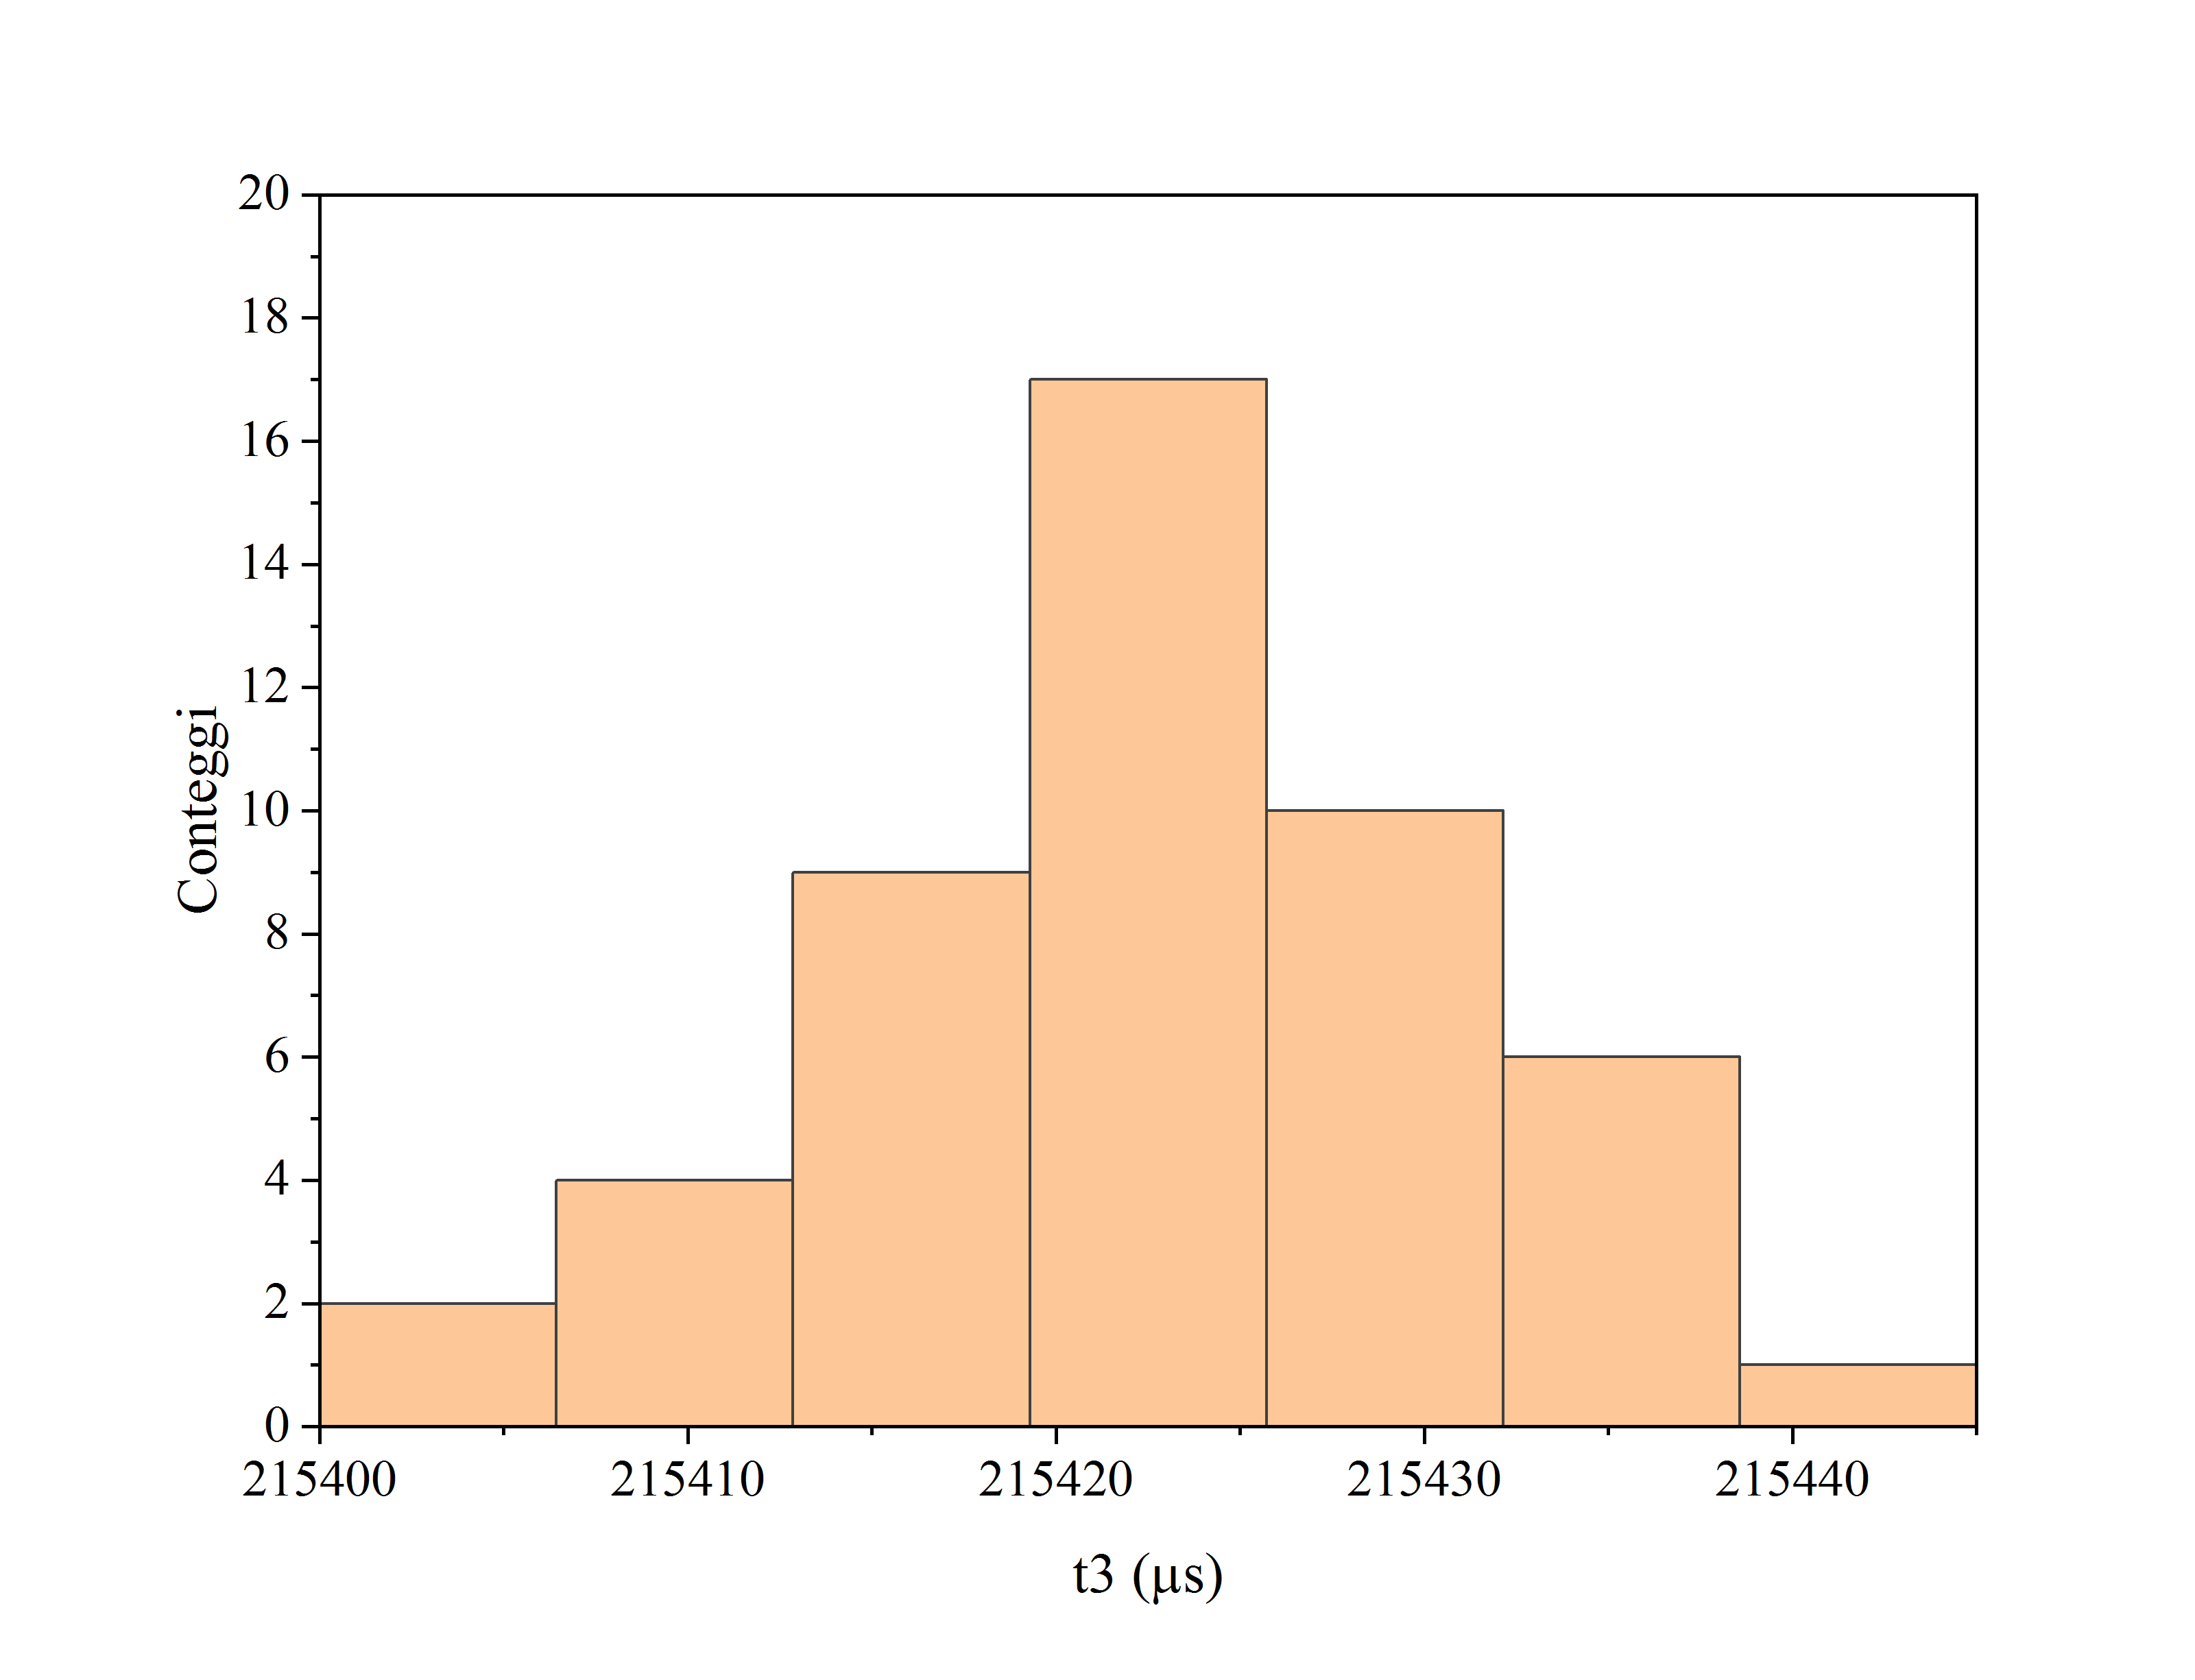
\includegraphics[trim={2cm .5cm 2.4cm 2.1cm},clip,width=.5\textwidth]{t3.jpg}
    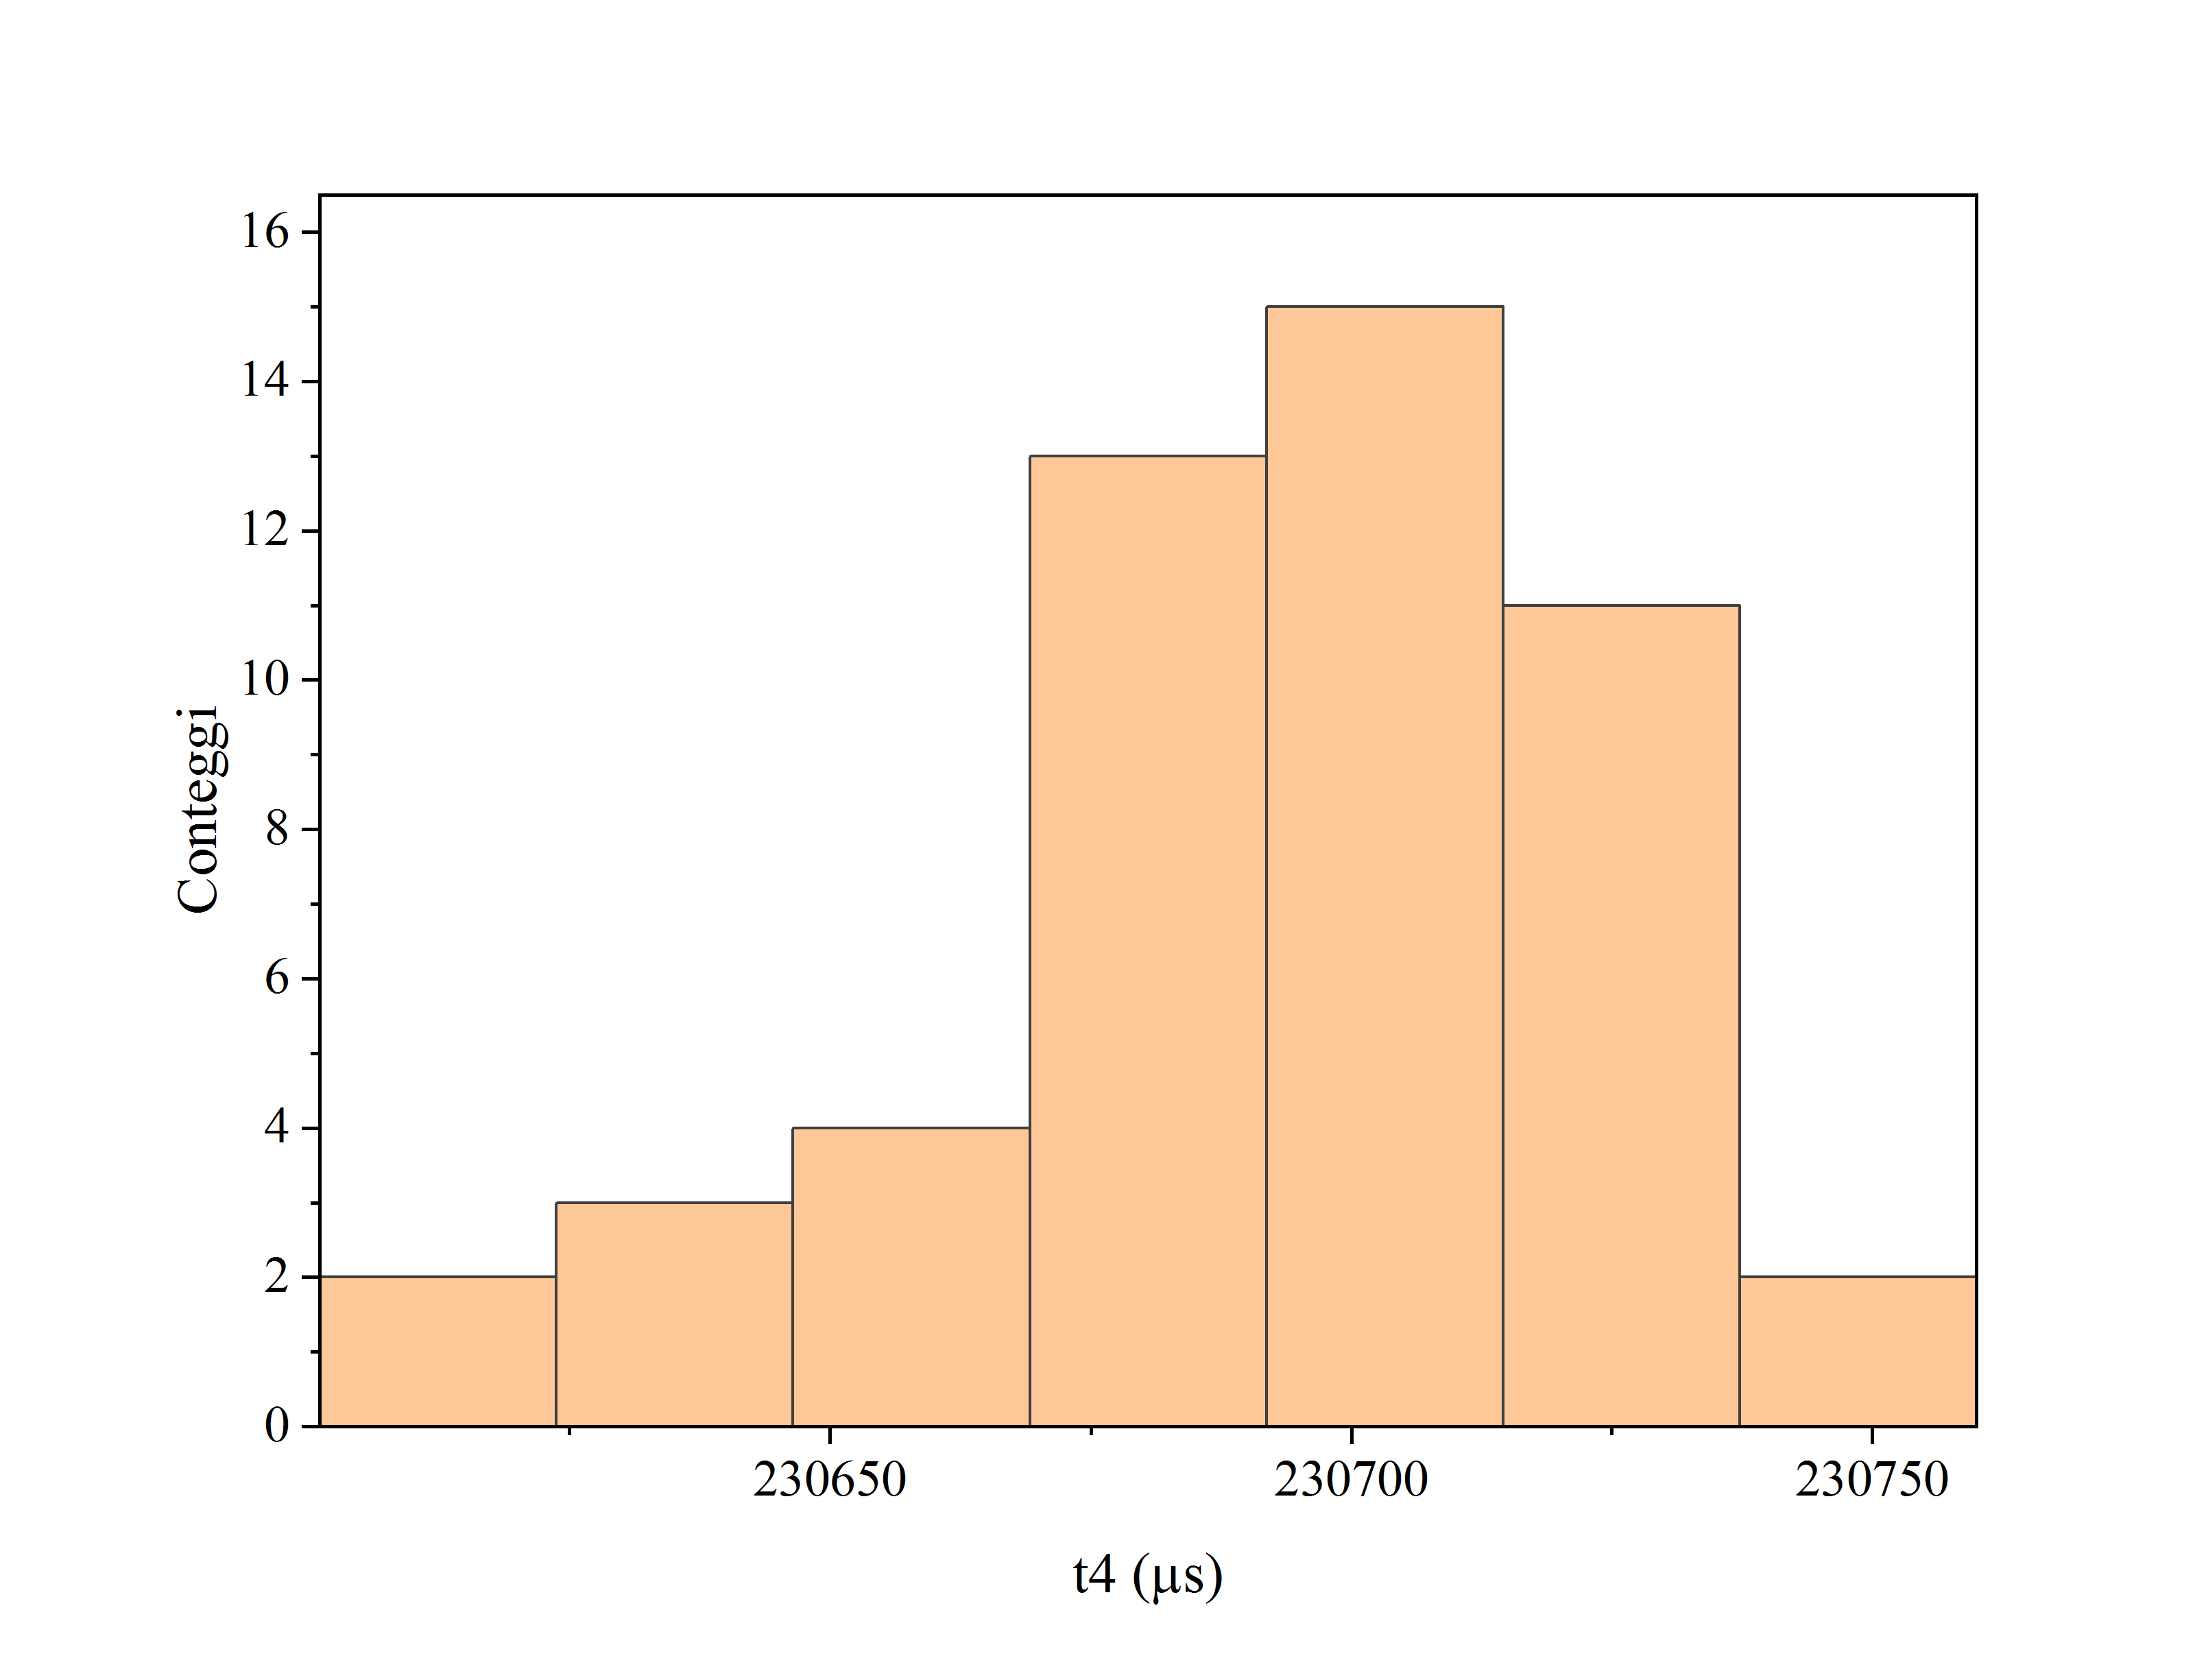
\includegraphics[trim={2cm .5cm 2.4cm 2.1cm},clip,width=.5\textwidth]{t4.jpg}
\end{figure}
\begin{figure}[H]
    \vspace{-.6cm}
    \centering
    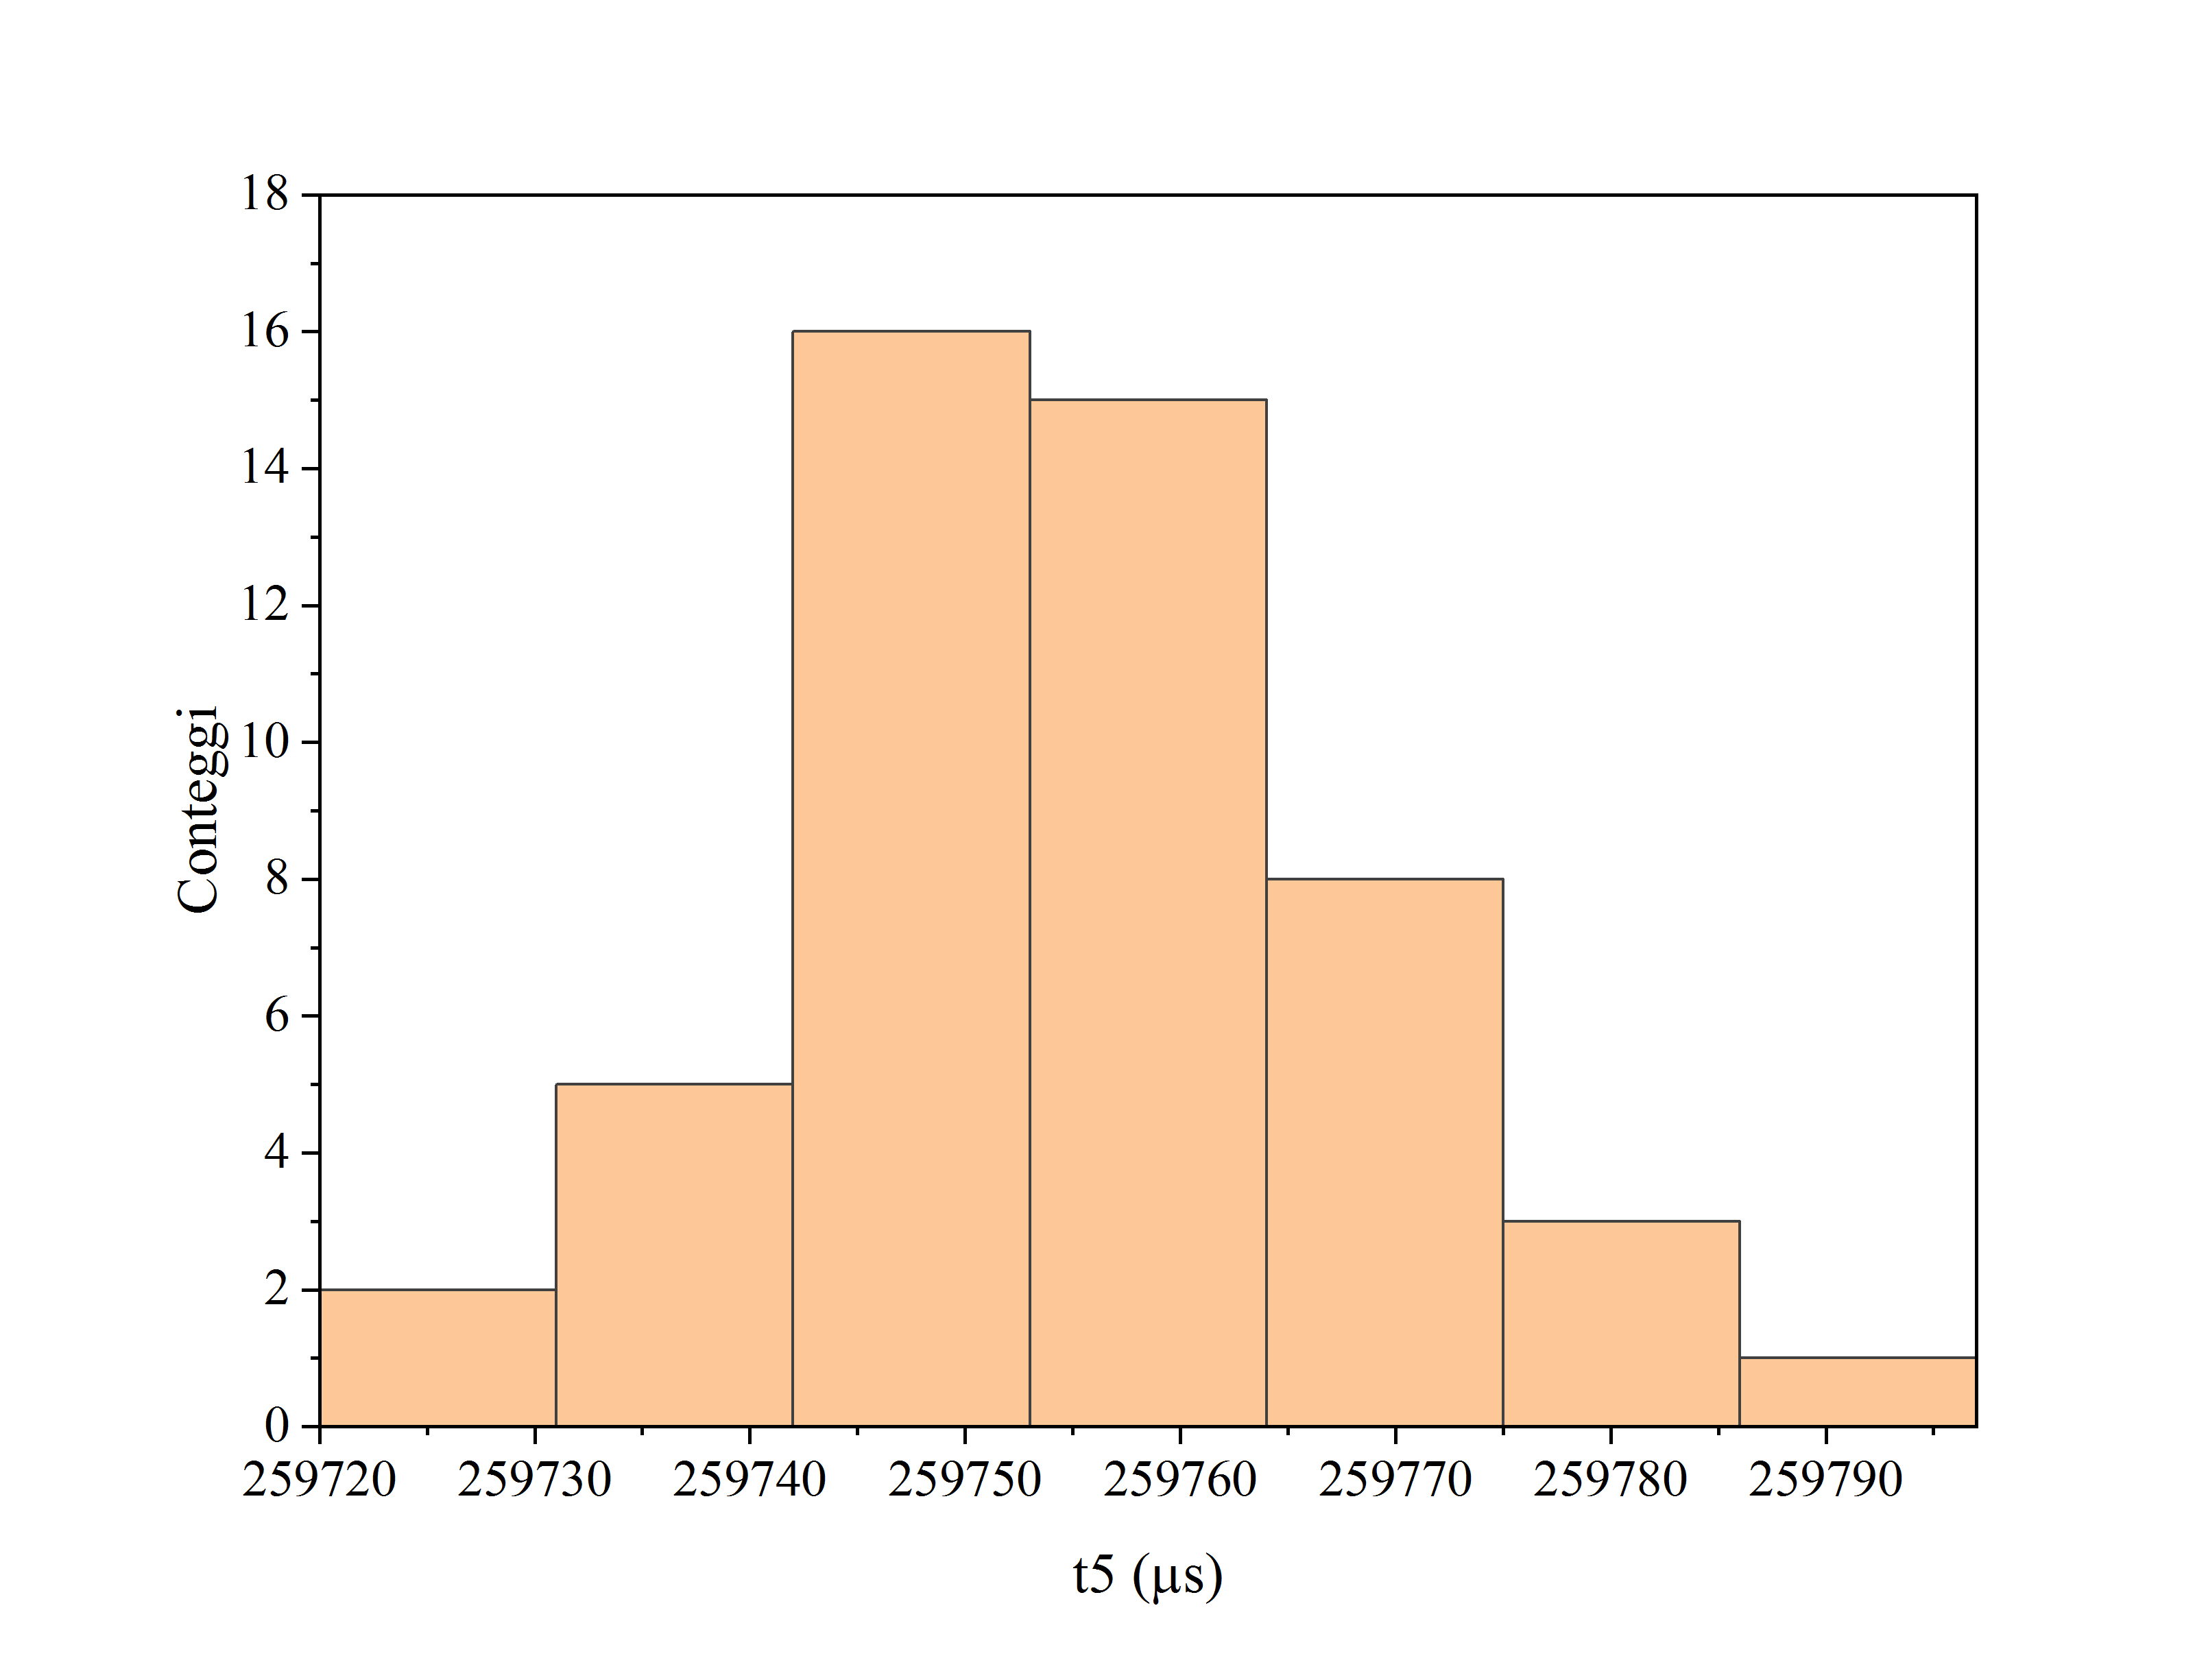
\includegraphics[trim={2cm .5cm 2.4cm 2.1cm},clip,width=.5\textwidth]{t5.jpg}
    \caption{Istogrammi dei tempi misurati ($t_1,t_2,t_3,t_4,t_5$)}
\end{figure}

\begin{center}
    \begin{tblr}{ |c|c|c|c| }
        \hline
            $i$ &
            $d_i\:(\unit{cm})$ &
            $\overline{t_i}\:(\unit{ms})$ &
            $\left(v_m\right)_i\:(\unit{m\per s})$ \\
        \hline
        1 & $ 53.3\pm0.1$ & $149.763\pm0.001$ & $3.559\pm0.007$ \\
        \hline[dashed]
        2 & $ 68.4\pm0.1$ & $183.710\pm0.001$ & $3.723\pm0.005$ \\
        \hline[dashed]
        3 & $ 83.6\pm0.1$ & $215.423\pm0.001$ & $3.881\pm0.005$ \\
        \hline[dashed]
        4 & $ 91.3\pm0.1$ & $230.694\pm0.005$ & $3.958\pm0.004$ \\
        \hline[dashed]
        5 & $106.5\pm0.1$ & $259.754\pm0.002$ & $4.100\pm0.004$ \\
        \hline
    \end{tblr}
\end{center}

\begin{figure}[H]
    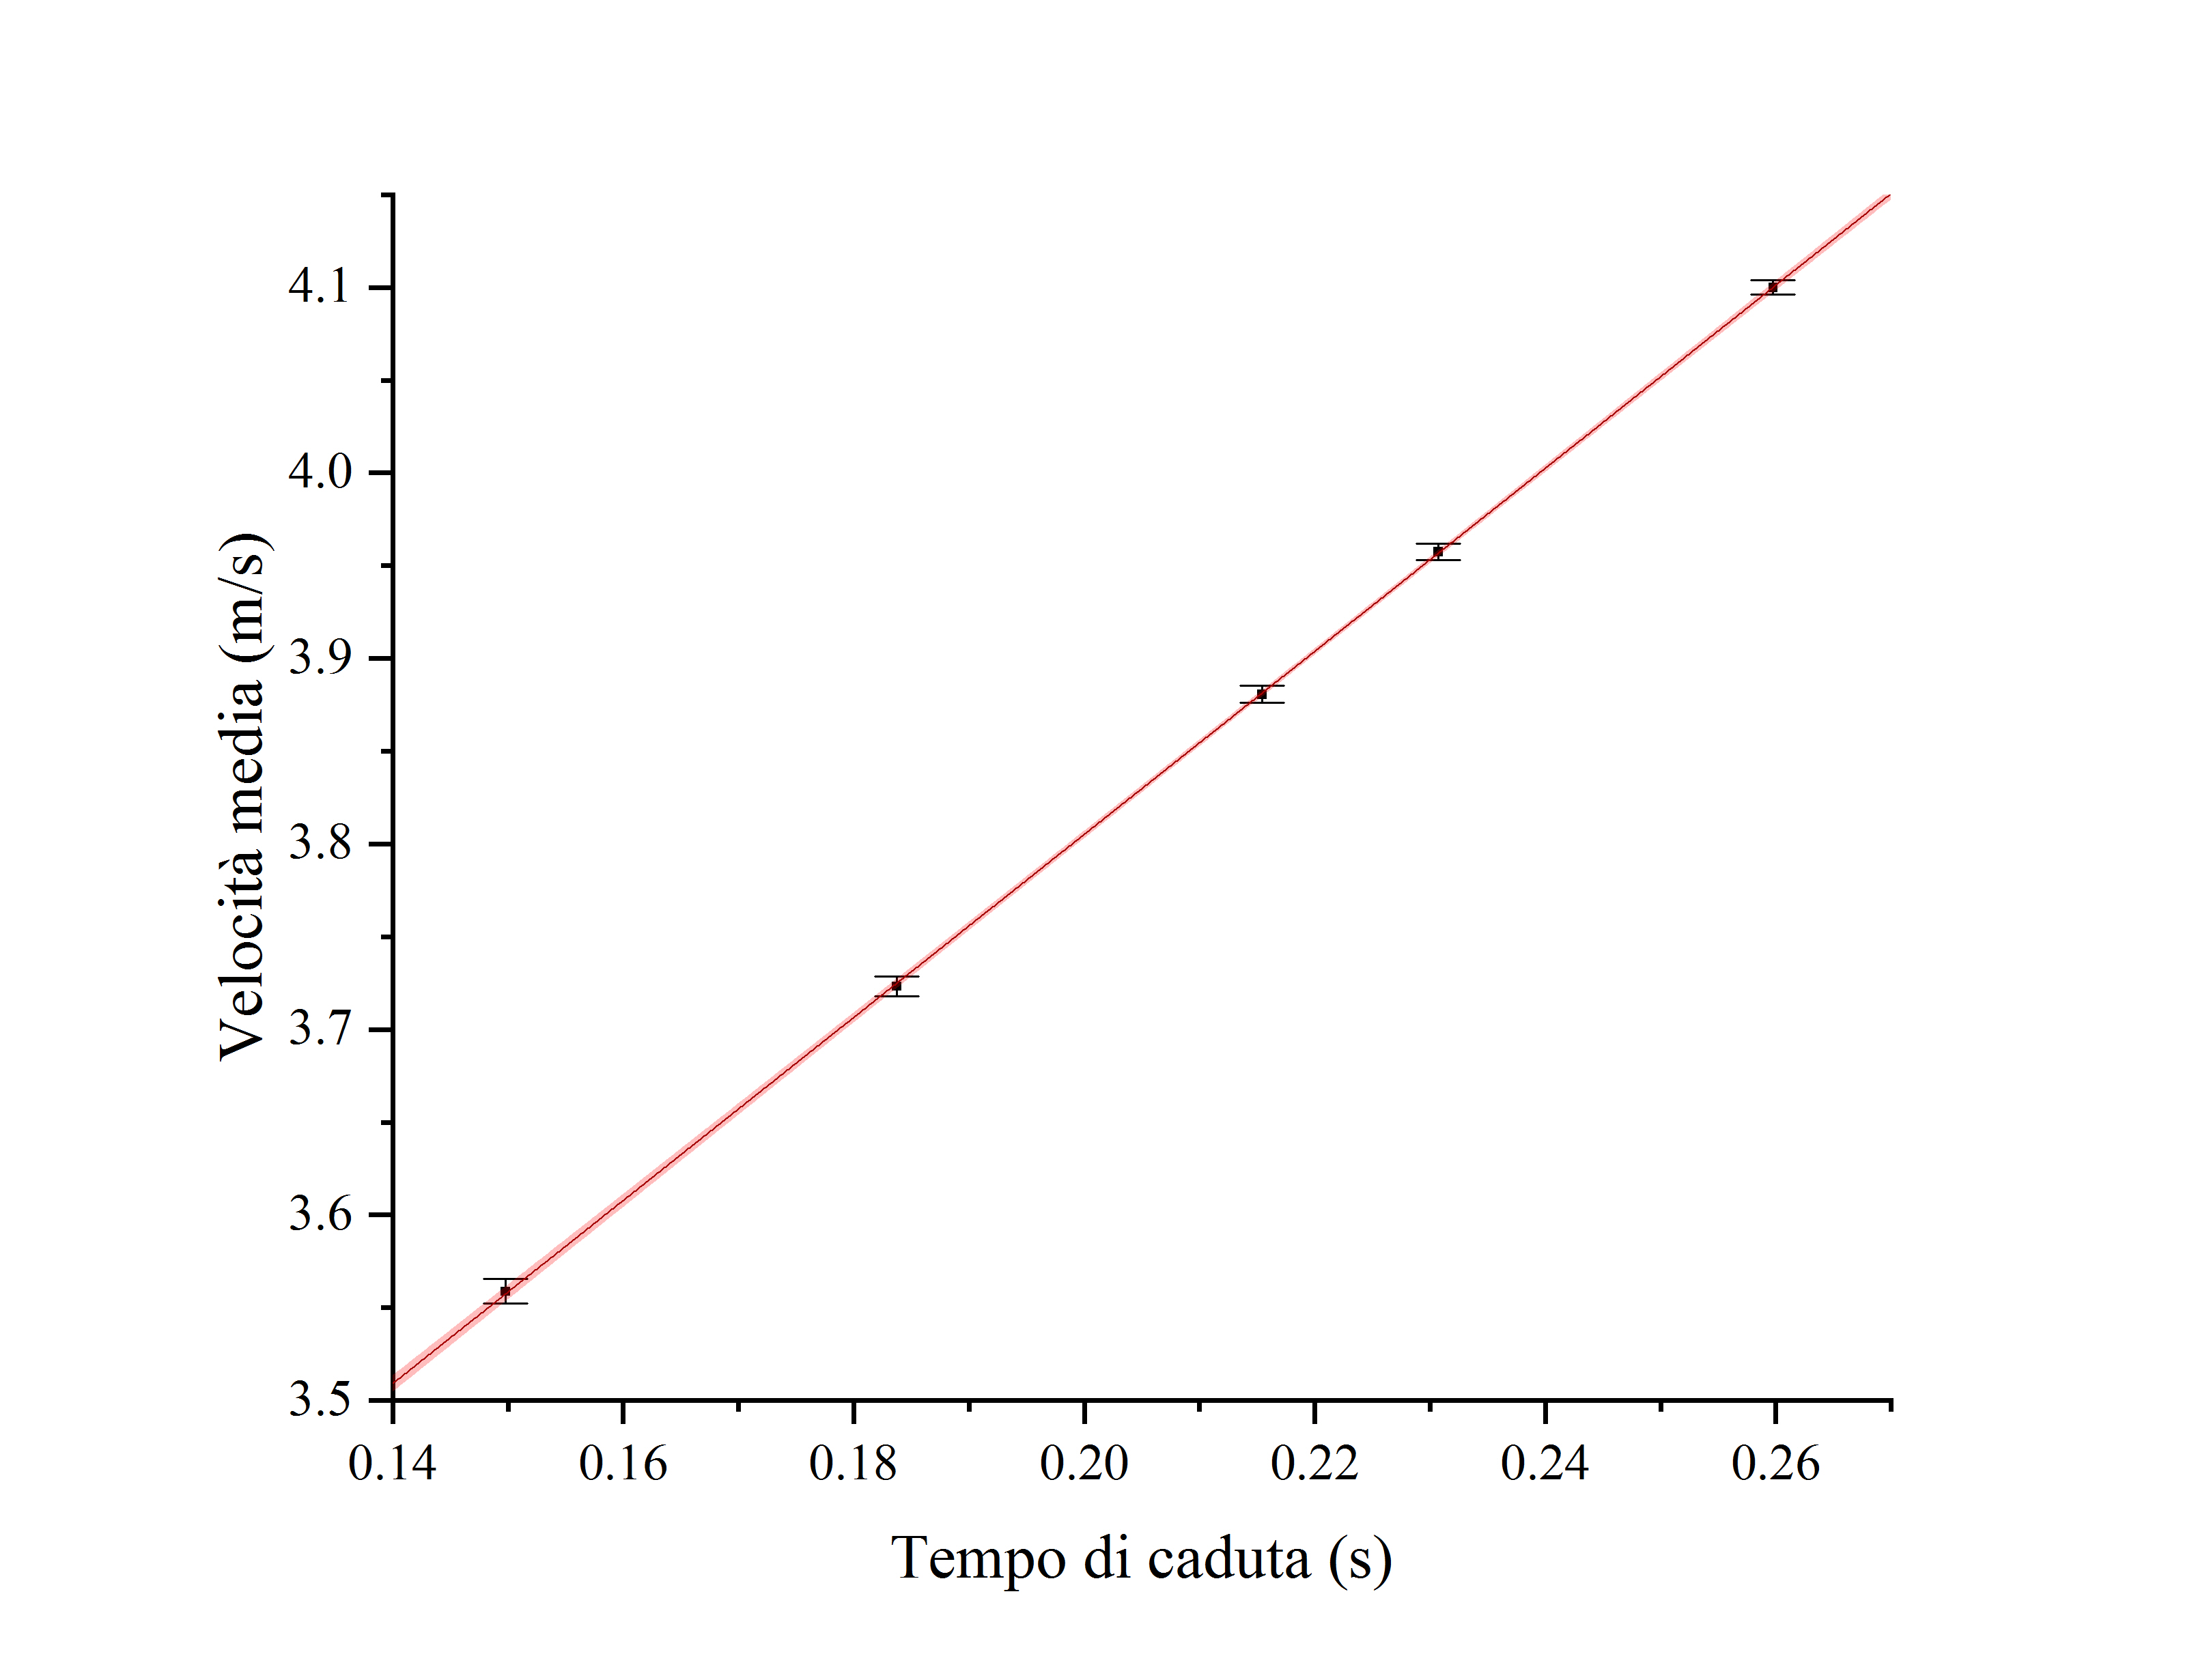
\includegraphics[trim={2cm .5cm 2cm 2.1cm},clip,width=\textwidth]{Regressione.jpg}
    \caption{
        La retta di regressione (in rosso) e la sua regione di incertezza (in rosa, appena visibile).
    }
\end{figure}

I risultati della regressione lineare sono i seguenti:
\begin{itemize}
    \item $v_0 = \left(2.818\pm0.014\right)\unit{m\per s}$ (del tutto sensato)
    \item $\frac{1}{2} g = \left(4.93\pm0.06\right)\unit{m\per s^2}$
    \item $g = \left(9.86\pm0.12\right)\unit{m\per s^2}$
\end{itemize}

Confrontiamo ora il $g$ misurato con il valore atteso
$\left(9.805 \pm 0.001\right)\unit{m\per s^2}$,
calcolando, come prima, il numero puro: \[
\varepsilon = \frac{\bestp{g_\text{misurato}} - g_\text{atteso}}{\delta g_\text{misurato}}
\]
Per noi, $\varepsilon = +0.45$, quindi la misura di $g$ che abbiamo
trovato è pienamente compatibile con il valore atteso.

\end{document}
